\documentclass{article}

\usepackage{graphicx}
\usepackage{hyperref}

\begin{document}
	
	\begin{titlepage}
		\centering
		\vspace*{3cm}
		
		
\includegraphics[width=0.4\textwidth]{images/fontyslogo.png} % Adjust the size of the logo
		\vspace{1.5cm}
		
		{\Huge\bfseries Personal Development Report}\\[1cm]
		{\LARGE Evaluation 3}\\[2cm]
		
		\textbf{Danil Burov}\\
		\vspace{0.5cm}
		\textit{Fontys University of Applied Sciences}\\[3cm]
		\vfill
		\textbf{\today}
		
	\end{titlepage}
	\newpage
	\tableofcontents
	\newpage
	
	\section{Introduction}
	My name is Danil Burov and I am studying Information Technology in Fontys, Venlo. I am specializing in 
	Embedded Software back in Venlo and the reason I chose this minor is because I think that AI is a very 
	ongoing topic and I wanted to get more familiar with it. Especially because I think that AI has a big 
	implication when it comes down to IoT devices.
	
	\section{Learning outcome 1 - Societal impact}
	\underline{\textbf{Description}}\\
	The student is able to approach the context and impact of their own AI project(s) 
	from different perspectives in a sustainable way. In addition, the student is able to 
	reflect on their own choices, taking into account data legislation and the (possible) impact on society.
	
	\underline{\textbf{Explanation:}}\\
	Societal impact is one of the most important contextual parts of the project. Every time a person 
	starts a project an evaluation on the societal impact should be done in order to understand 'Why?'
	a project is being done on the given topic.
	
	\subsection{First evaluation}
	During the first weeks of the minor I had the opportunity to think about the societal impact of the projects I will 
	be working on. Since the beginning I had an idea of what my personal project could look like. However, I was not that aware
	what could be the societal impact of my project. With the help of the technical coach 'Jacco' I established an understanding what
  could be a potential idea. The feedpulse submission will be shown under:\\
  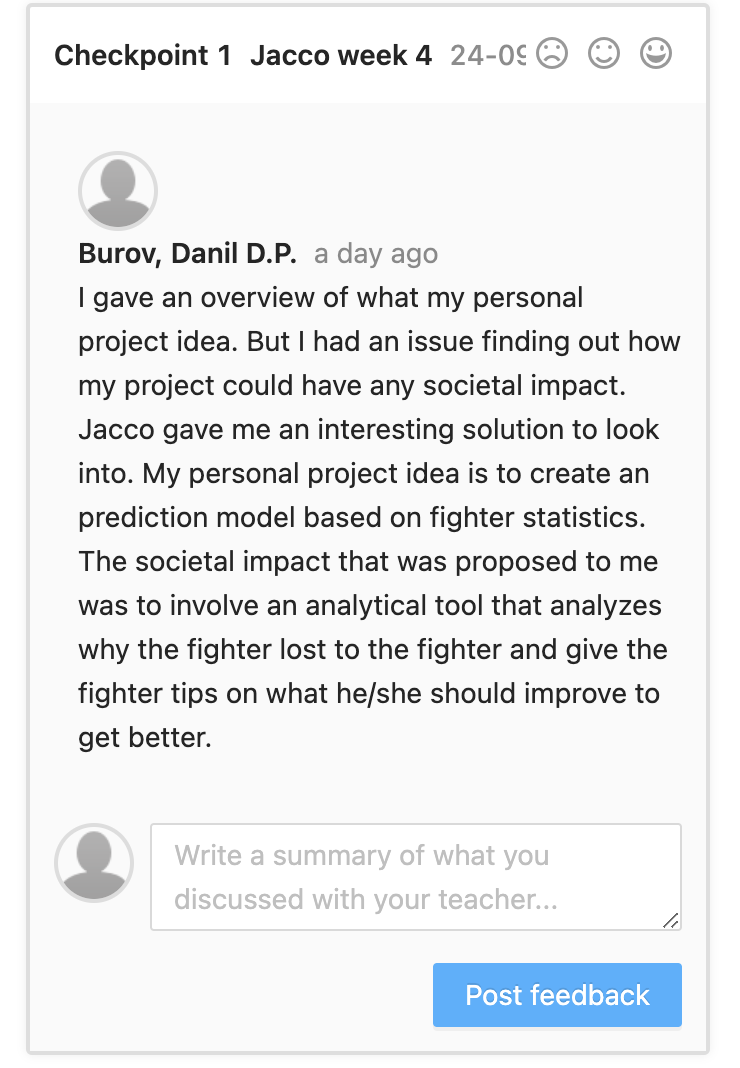
\includegraphics[width=\textwidth,keepaspectratio]{images/Feedback_Societal_Impact.png}
	
	\underline{\textbf{Self assessment: Orientating}}
	
	\subsection{Second evaluation}
	From week six to week nine I did not really improve on my societal impact learning outcome. This is mainly due to the reason that 
	I was mainly focusing on modelling my first model and learning how to prepare data for training. In the upcoming weeks I will make sure that 
	I take time as well to work on the societal impact goal as well, starting with writing the 'Potential Impact Assessment'.
	
	\underline{\textbf{Self assessment: Orientating}}
	
	\subsection{Third evaluation}
	During the third evaluation of my project, I delved deeper into analyzing the potential societal impact it might have. With the guidance of my teacher, Niek, I was able to create a solid first draft of the impact analysis. Niek has been a consistent source of support since I began working on this document, helping me navigate its purpose and structure.\\
	
	Initially, I struggled to see the relevance of creating an impact analysis. It seemed like an unnecessary artifact. However, as I started writing and consulting with Niek, I began to recognize its significance. The process encouraged me to critically consider the potential impact of my project on various societies, as well as on the individuals whose data I am analyzing and using to train the model. Niek’s advice to clearly define the purpose of any document proved invaluable. This guidance not only helped me articulate the intent of the impact analysis but also 
	improved its overall quality and focus.\\
	  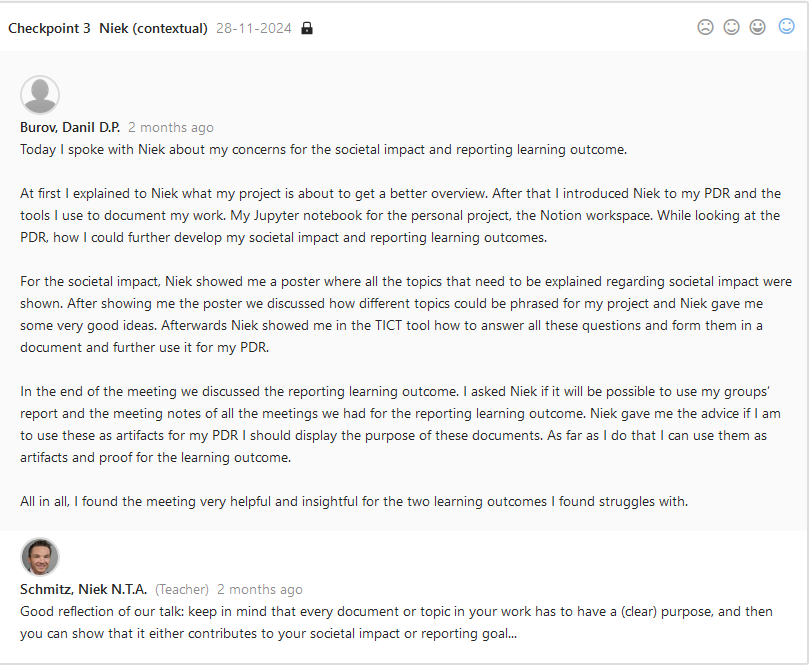
\includegraphics[width=\textwidth,keepaspectratio]{images/Feedback_Niek_1.png}\\
	
	Despite this progress, I encountered challenges, particularly in aligning the context of my project with the purpose of the analysis. While I understood the document’s goals and expectations, addressing the topic of energy consumption proved difficult. I wasn’t entirely sure what was required or how to approach it. Niek’s support was crucial here; he helped clarify the energy consumption topic, enabling me to tackle it with a better understanding.
	
	In the first draft of the impact analysis, I was confident that my project should remain strictly private. However, during a feedback session with Niek, he raised a compelling point that challenged my perspective on privacy. His insights made me reconsider my initial stance and reflect more deeply on the broader implications of privacy in my project.\\
  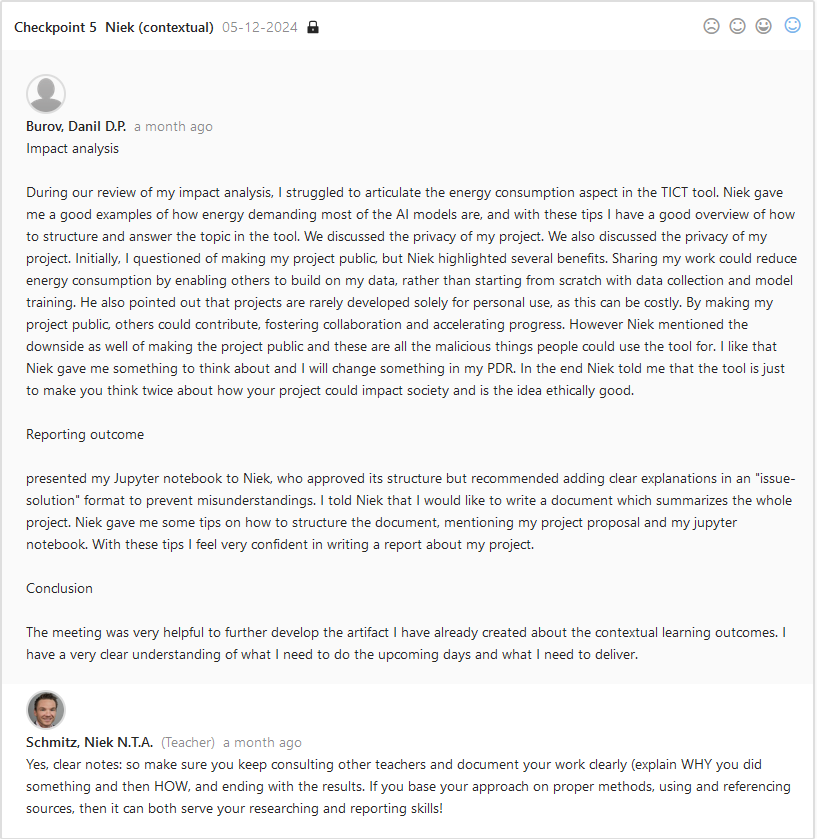
\includegraphics[width=\textwidth]{images/Feedback_Niek_2.png}\\\\
	Since then, I have continued to refine the impact analysis. I’ve been experimenting with different approaches, seeking feedback, and iterating on the document. This process has extended into the fourth quarter, and I’m committed to further improving the analysis to ensure it accurately captures the societal impact of my work.\\
	  \underline{\textbf{Self assessment: Beginning}}
	\subsection{Final evaluation} %AFTER NIEK FEEDBACK
	\underline{Self assesment: Proficient}
	
	\section{Learning outcome 2 - Investigative problem solving}
	\underline{\textbf{Description}}\\
	The student is able to critically look at their own AI project(s) from different perspectives, 
	recognize problems and come up with appropriate solutions.
	
	\underline{\textbf{Explanation:}}\\
	From this learning outcome I will further develop my investigative and problem solving skills regarding 
	how AI is used in the project, is it doing as intended and if not how to approach the problem and solve it 
	eventually.
	
	\subsection{First evaluation}
	During the first weeks I had to tackle several problems. In the beginning, the course was presented with some stakeholders 
	who presented to us what issues they have with their companies and what they would like to add to their business. I was given 
	the opportunity to think of an idea that solves a business case and so I created a project proposal for one of the companies that visited us. 
	The proposal is based on the problem that the company has.
	
	To see the full proposal go to this link: \href{https://github.com/BurovDanil/MinorAI/blob/main/Documents/Project%20Proposal/Proposal.md}{project proposal}
	
	\underline{\textbf{Self assessment: Orientating}}
	
	\subsection{Second evaluation}
	I have been dealing with a legal issue for the past weeks because, for my personal project, I would love to have as much actual data as possible. 
	In order to do that, I needed to develop a scraper for the websites' statistics. Before doing so I checked the terms and conditions of the website. 
	Unfortunately, the website forbids any scraping and bots developed for the purpose of gathering data. So I investigated a way to still be able 
	to scrape the data and use it for my personal project. In the upcoming weeks I will create a document where I explicitly say what is the intended usage of 
	my project and why the scraper was developed.
	
	\underline{\textbf{Self assessment: Beginning}}
	
	\subsection{Third evaluation}
	During this quarter of the semester, I also encountered challenges with my personal project, particularly in data preparation, analyzing societal impacts, and choosing a model for the data. Writing the societal impact analysis required me to deeply consider who might use my project and how it could potentially be exploited. This exercise helped me brainstorm solutions to mitigate these risks. It also encouraged me to think about the broader future impact of my project, both positive and negative.\\
	
	Regarding data preparation, I dealt with a significant amount of unstructured data that required cleaning and organizing for modeling. With the guidance of my semester coach, I successfully created a well-structured and cleaned dataset, ready for modeling.\\
	  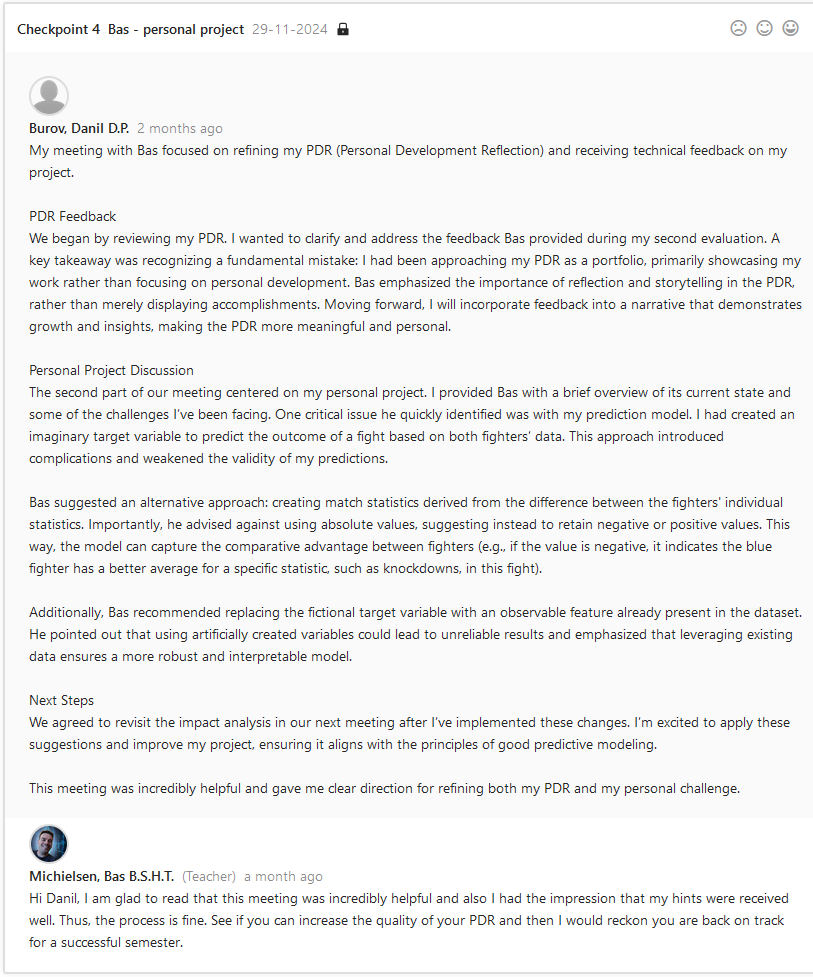
\includegraphics[width=\textwidth]{images/Feedback_Bas_1.png}\\
	
	Choosing a model proved to be the most challenging aspect for me. I struggled because I needed to understand the underlying technology and how it aligned with my project’s goals. Through extensive self-research and discussions with Bas, I realized that selecting a model should not be the immediate priority. Instead, Bas emphasized the importance of building a robust dataset first. As he put it, "Don’t rush into modeling; focus on creating a strong dataset, and the modeling will follow." This advice shifted my perspective and made the task feel more manageable.\\
	  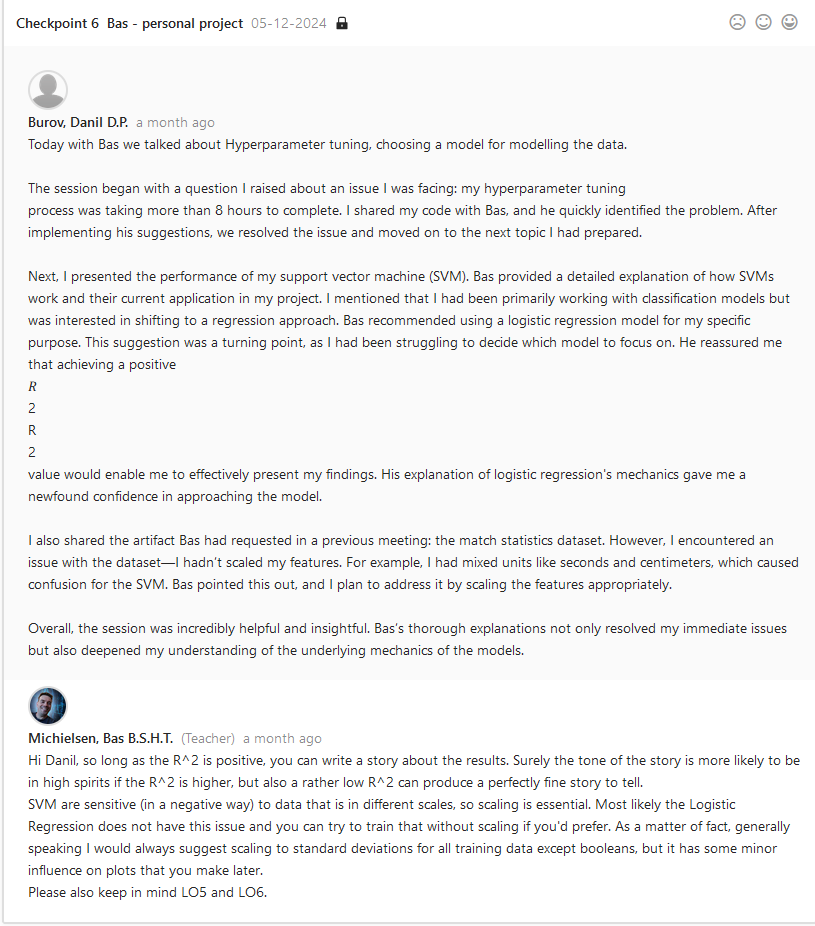
\includegraphics[width=\textwidth]{images/Feedback_Bas_2.png}\\
	
	I’m excited about the upcoming challenges in the final quarter of the semester. I feel like I’m on the right track and look forward to tackling new problems and learning from them.\\
	  \underline{\textbf{Self assessment: Beginning}}
	\subsection{Final evaluation} %AFTER NIEK FEEDBACK
	\underline{Self assesment: Proficient}

	\section{Learning outcome 3 - Data preparation}
	\underline{\textbf{Description}}\\
	The student is able to collect data and estimate its quality and usability. 
	The student is also able to adjust the data if necessary for proper usage in their project(s).
	
	\underline{\textbf{Explanation:}}\\
	In order to create any AI model I will need a good, clean dataset that can be used to properly teach a machine.
	To do so I intend to first of all use a reliable source for the set and inspect it carefully before using.
	
	\subsection{First evaluation}
	The first thing that was done regarding this learning outcome was to select a dataset suitable for the intended usage of the 
	AI model. For the personal project I have selected this \href{https://www.kaggle.com/datasets/asaniczka/ufc-fighters-statistics}{dataset}. I have been working on a cleaned version of this dataset. 
	Since this dataset does have some empty fields I tried already cleaning some of the data to prepare it for the upcoming modeling. Regarding the data preparation 
	for the project, I have already started analyzing the data for the organization we are doing the project for, however it is still in a very early stage.
	
	\underline{\textbf{Self assessment: Orientating}}
	
	\subsection{Second evaluation}
	I have been preparing data for the past couple of weeks for both my personal and group projects. In the past weeks in the group project, I have been 
	trying to estimate the quality and the usability of the data that was provided by our stakeholder. To assess the quality and usability I cleaned 
	the data from any 'null' fields and factorized some of the features. I also combined features into a new feature. Especially in my personal 
	project, I had to check each fighters' statistics and based on them I labeled the fighters' fight style.
	
	\underline{\textbf{Self assessment: Beginning}}
	
	\subsection{Third evaluation}
	Since the last evaluation, I feel I have significantly improved in the data preparation outcome. My semester coach and I have worked extensively with a semi-large dataset that contained many unnecessary features. At the beginning of the minor, I wasn’t entirely sure what cleaning data entailed. However, I now feel confident in how to approach and start this process. That said, I acknowledge there’s still much to learn.\\
	
	In my most recent feedback session with my coach, a major issue in my dataset was identified: I hadn’t applied standard deviation, which left certain numerical values (e.g., seconds and centimeters) unnormalized. This oversight was particularly problematic for models like Support Vector Machines, which require properly cleaned data to perform well. This feedback session taught me the importance of always double-checking my work, even when I feel confident in its accuracy. I also learned that the quality of the dataset directly determines the model’s performance.\\
	
	 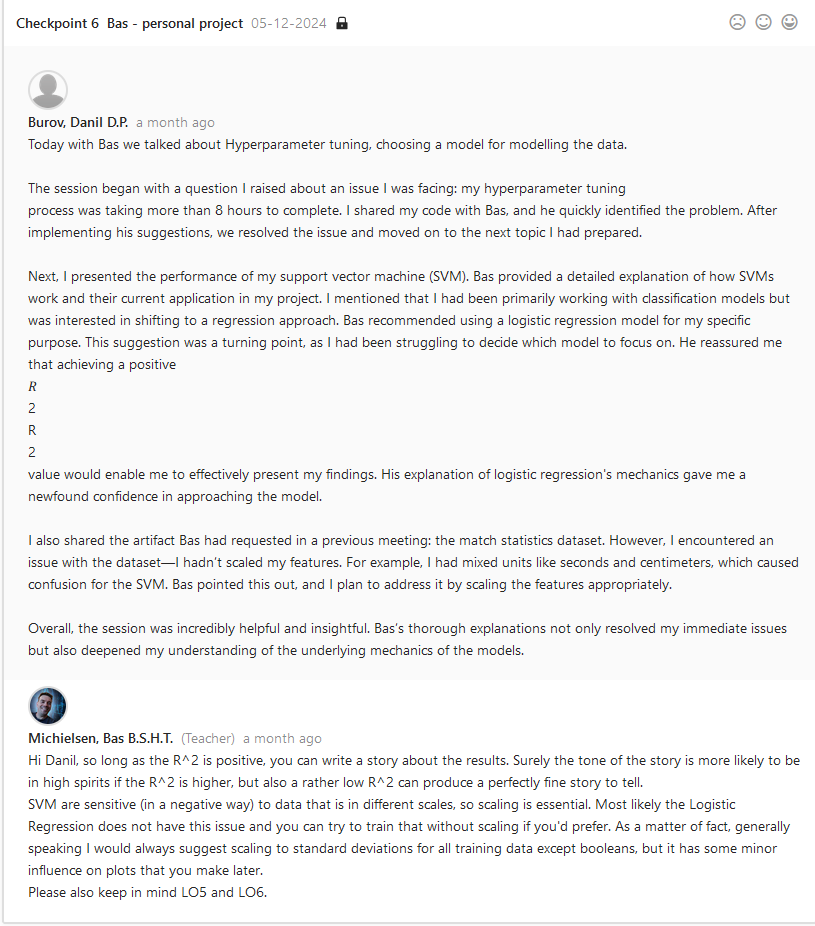
\includegraphics[width=\textwidth]{images/Feedback_Bas_2.png}\\
	
	Bas gave me a valuable analogy that stuck with me: “You can modify a coffee machine as much as you want, but if the coffee itself is bad, the result will always be bad.” This lesson reinforced the idea that a high-quality dataset is the foundation of successful modeling. I’ve internalized this insight and will prioritize ensuring my datasets are robust before moving forward with modeling.\\
	  \underline{\textbf{Self assessment: Beginning}}
	\subsection{Final evaluation}
	In the last quarter of the semester I looked further into the dataset I was using for my models. I established based on a previous feedback with my semester coach Bas, that the data I currently have is too incomplete or not good enough to model it.\\\\
	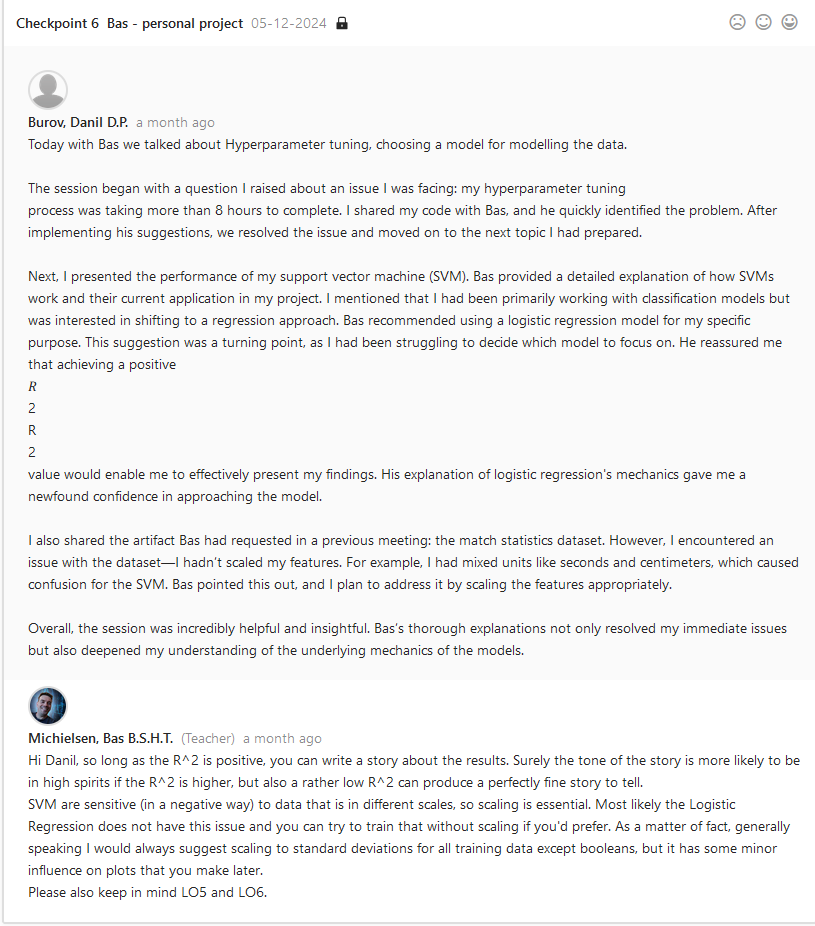
\includegraphics[width=\textwidth]{images/Feedback_Bas_2.png}\\
	To address this issue I decided to train a model on a different dataset, which was a combination between the whole match history of all the bouts in the UFC and all the fighter specific data. I managed to merge these two datasets and derive from each fighters statistics for a match, the difference between their statistics. This felt like a better set for modelling.\\\\
	Unfortunately, I have not received any feedback on the dataset preparation since I was focusing on other learning outcomes more.
	\underline{Self assesment: Proficient}
	
	\section{Learning outcome 4 - Machine teaching}
	\underline{\textbf{Description}}\\
	The student is able to use data to train models in a way that fits the intended purpose.
	The student is also able to test whether the models have been adequately trained.
	
	\underline{\textbf{Explanation:}}\\
	After making sure that the dataset that will be used to teach a machine is not corrupted, outdated, etc., 
	I need to ensure that the machine is doing as intended with the dataset. In order to ensure quality, testing the
	machine teaching is ideal.
	
	\subsection{First evaluation}
	In the first weeks of the minor I explored a website called 'Teachable Machine' in order to get familiar with the steps of creating an 
	AI model. The usage of my model was to recognize cats and dogs.Other than using the website to get familiar with machine learning, 
  I have tried to familiarize myself with different machine learning algorithms, such as Decision Trees, Random Forest, etc. Here you can see the received feedback from one
  of my lectures:\\
  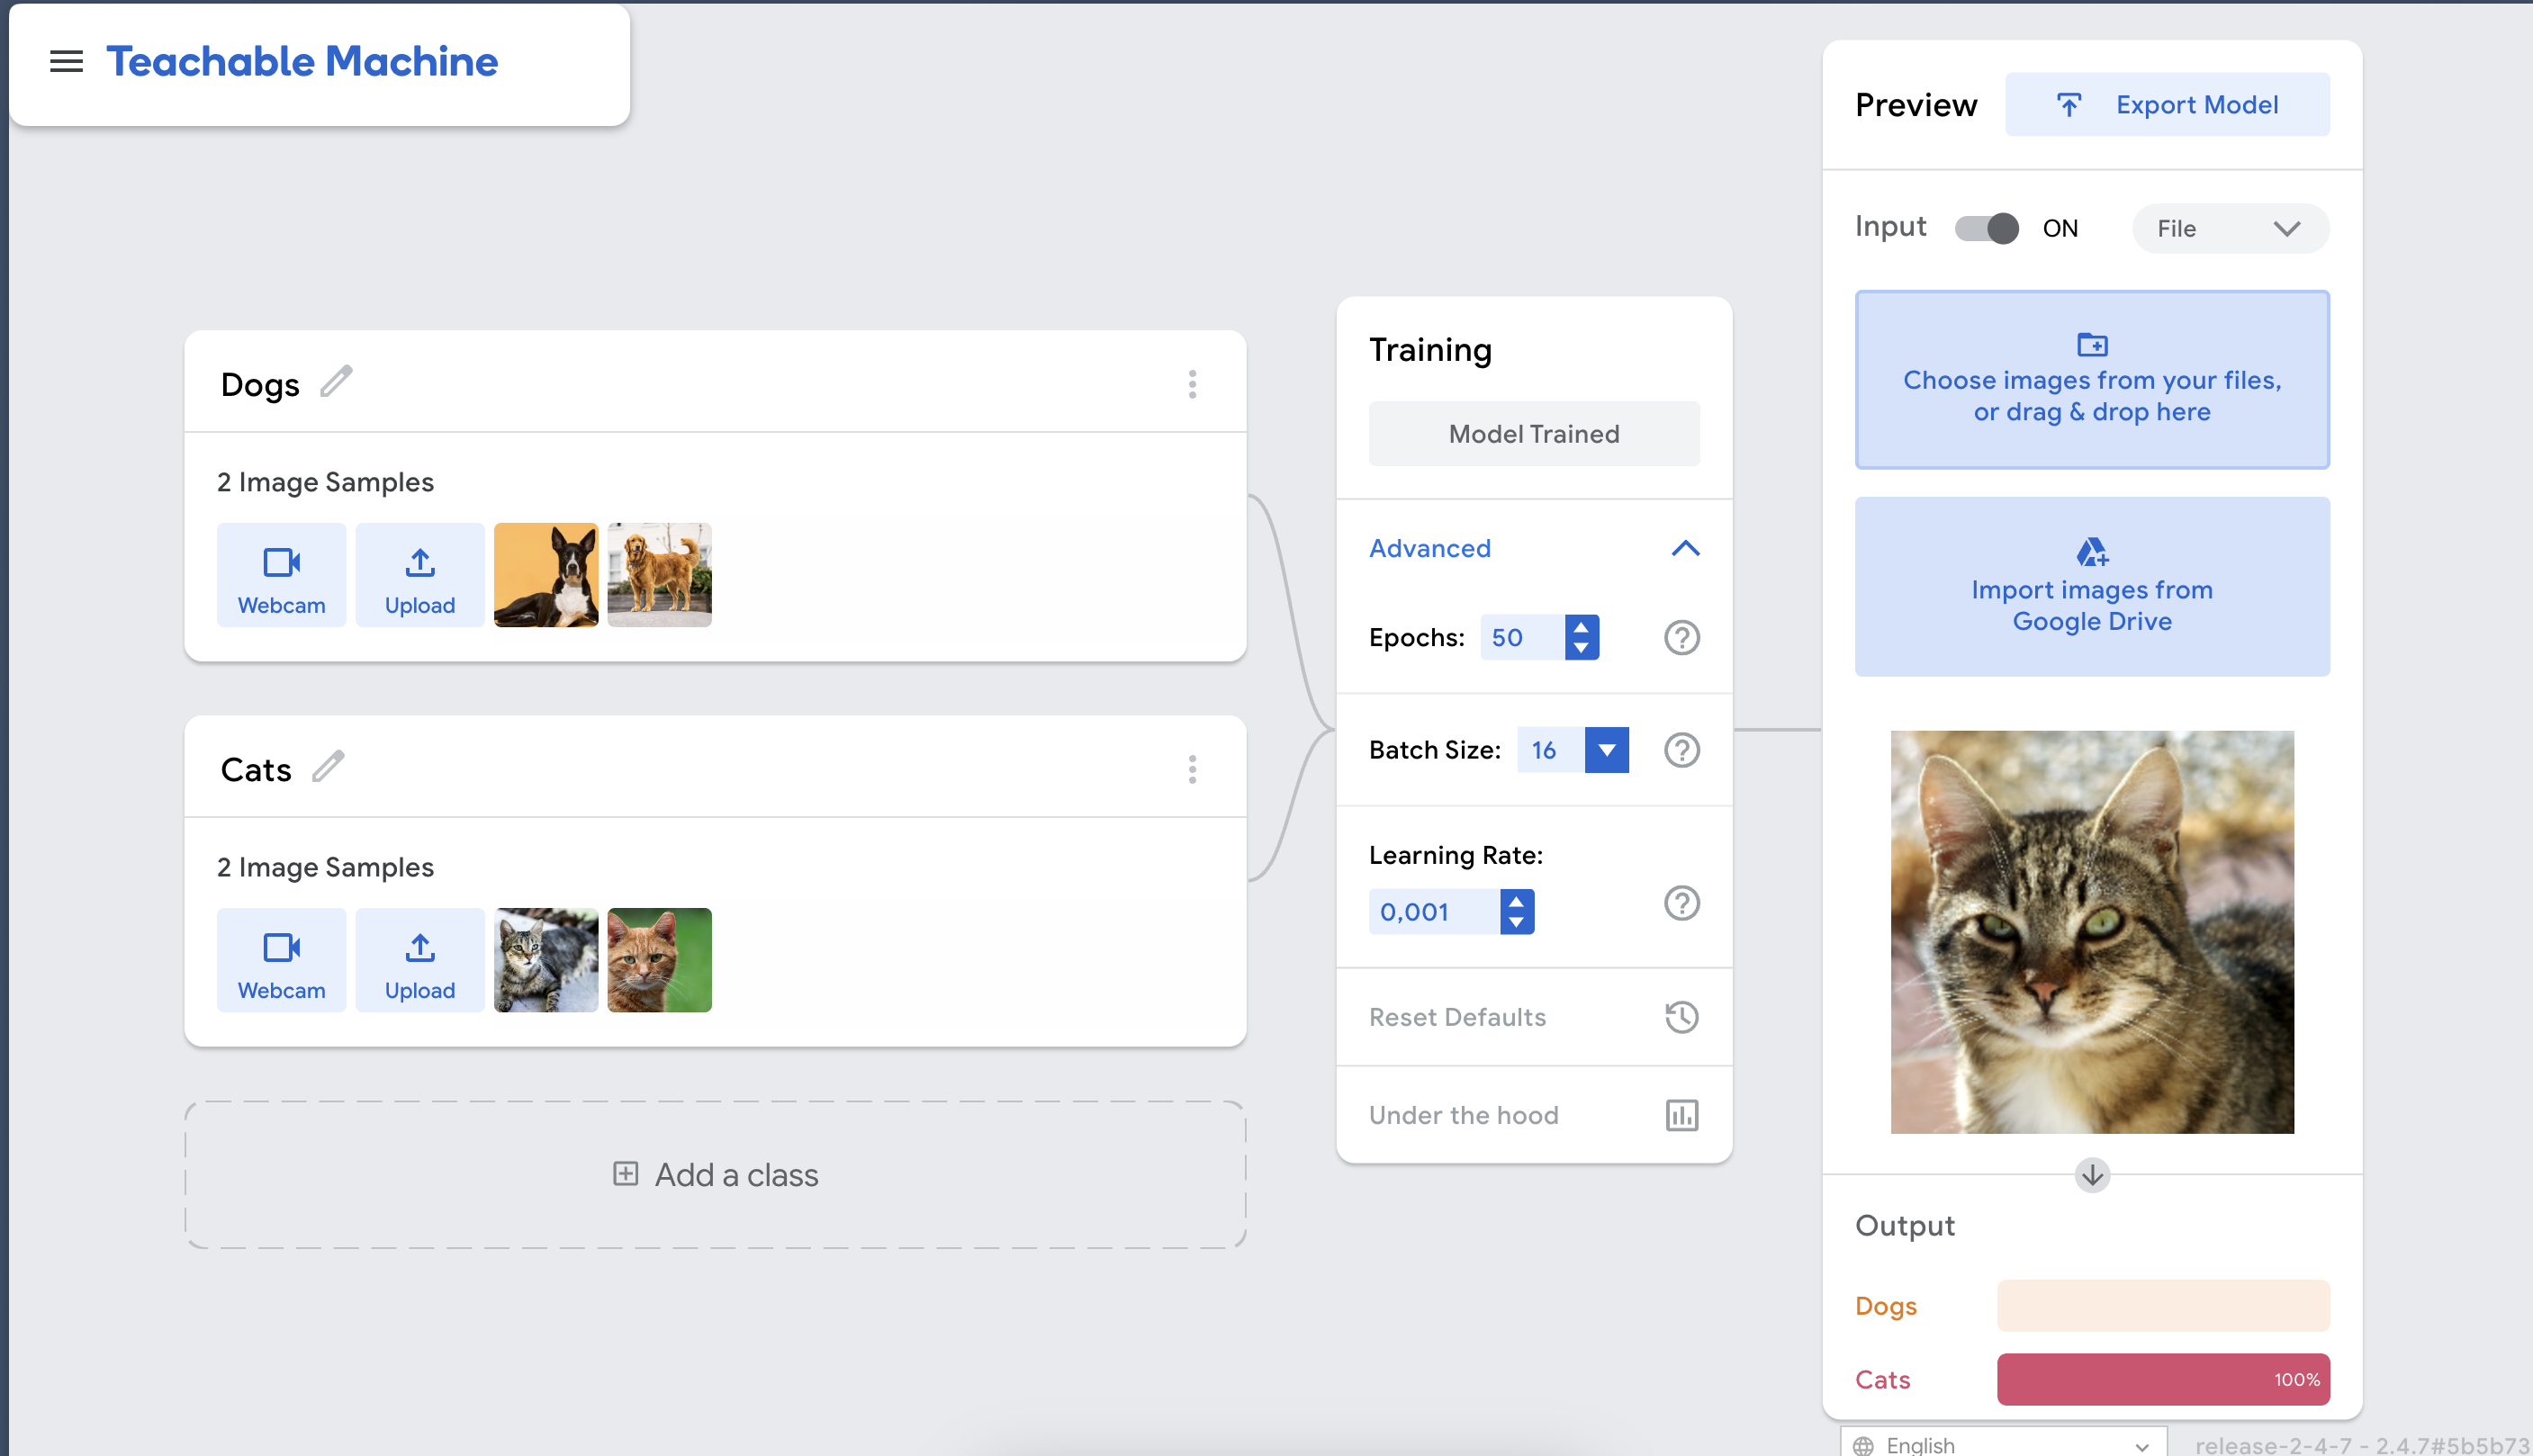
\includegraphics[width=\textwidth,keepaspectratio]{images/FeedbackTeachableMachines.png}

  \underline{\textbf{Self assessment: Orientating}}

	\subsection{Second evaluation}
	I managed to model the data of my personal project, whereas in my group project I mainly analyzed and cleaned the data. The difficulties
	I found along the way were mainly choosing the model that was actually fitting the purpose of my project. I had to choose between a 'Classifier'
	and a 'Regressor' first. For my personal project, I chose to use the 'Random Forest Classifier' model, because I was mainly trying to have a 
	prediction of yes or no. However, after my meeting with my semester coach Bas I decided to redirect my focus on actually estimating 
	the likelihood of each fighter winning a match against each other. The upcoming weeks I will be trying to teach a model with the data I have
  analyzed in my project.
	
  \underline{\textbf{Self assessment: Beginning}}
	
	\subsection{Third evaluation}
	Machine teaching remains one of the learning outcomes where I feel I still have significant room for improvement. Personally, I find it challenging to teach a machine using a model that I do not fully understand. Fortunately, my semester coach, Bas, has been instrumental in helping me deepen my understanding of why certain models are better suited to specific situations.\\
	
	In my last feedback session with Bas, I implemented a Support Vector Machine (SVM) for my personal project. However, Bas quickly pointed out that this model would not perform well given the dataset and the objectives of my project. He explained the underlying mechanics of SVMs and why they were not an optimal choice in this scenario. After our discussion, we concluded that Logistic Regression would be a more suitable option. This decision was based on how Logistic Regression operates, which aligns better with the characteristics of my data and the project's purpose.\\
	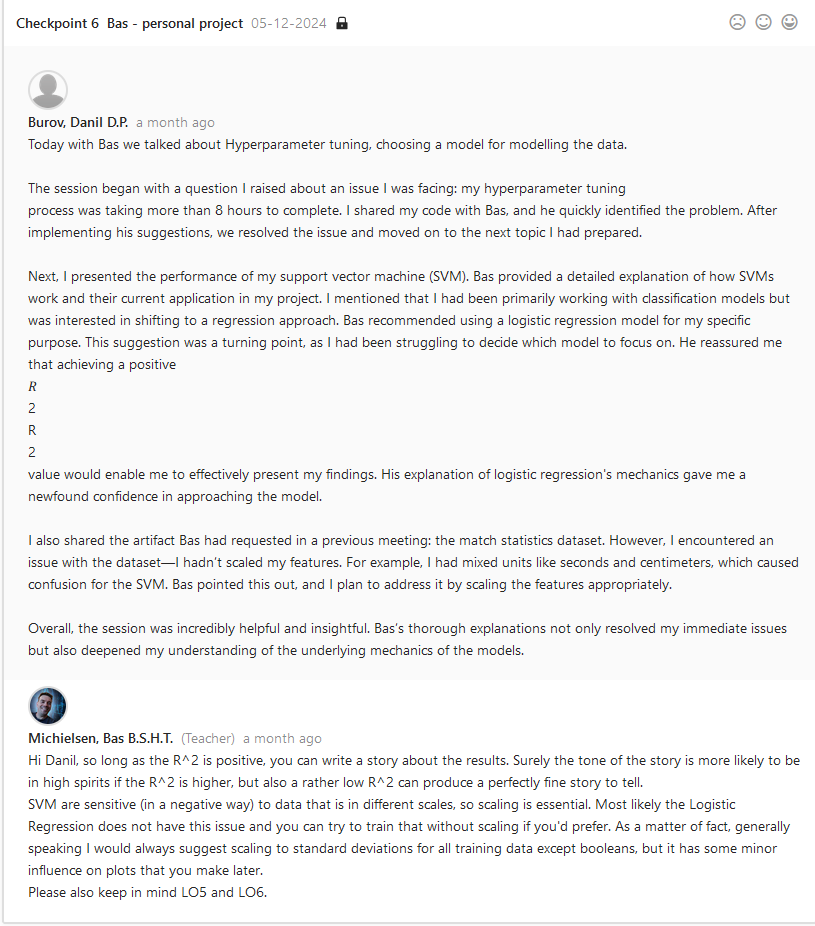
\includegraphics[width=\textwidth]{images/Feedback_Bas_2.png}\\
	
	
	At the start of my project, my goal was to use a classification model to output binary results, such as 0 or 1, with no values in between. My initial idea was to predict which fighter would win a match. However, after multiple discussions with teammates and Bas, I realized that regression modeling was a better fit for my case. Regression models differ in that they don’t provide an accuracy score; instead, the output itself represents the model's prediction accuracy.\\
	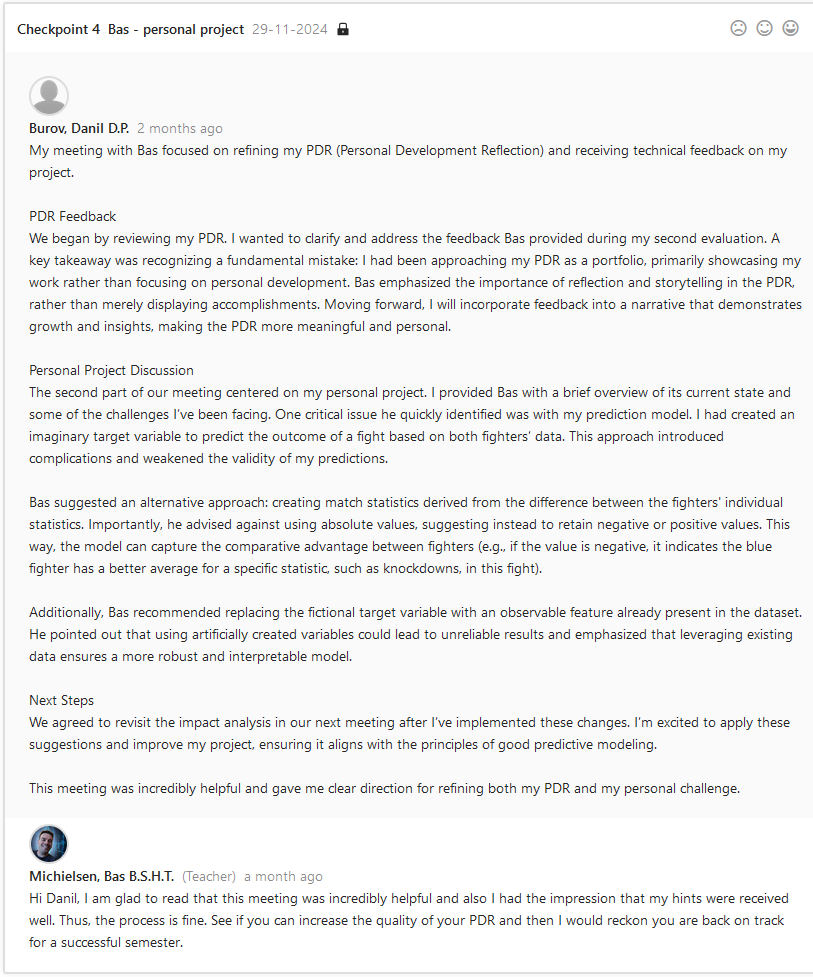
\includegraphics[width=\textwidth]{images/Feedback_Bas_1.png}\\
	
	This shift in approach was particularly enlightening. It is almost impossible to collect data and train a model to accurately predict fight outcomes because human factors are inherently unpredictable. With regression, the goal is not to predict a binary result (win or lose) but rather to produce a continuous range of values that capture all possibilities in between. This approach aligns perfectly with my use case and has given me a deeper appreciation for the nuanced applications of machine teaching.\\
	  \underline{\textbf{Self assessment: Beginning}}
	
	\subsection{Final evaluation}
	The shift that I had to make since the last evaluation has been rather fun to adjust. I have been trying to model the data with Logistic Regression ever since. In the beginning I created a target variable which was a combination of all the targets I wanted to predict (KO/TKO, Winner, Submission and unanimous decision prediction for a bout). However, Bas once told me it is not a good idea to create your own target variable but rather use an exisiting feature and not include in the training and testing sets. Based on this feedback I decided that I will need to have 4 different models to predict the different outcomes.
	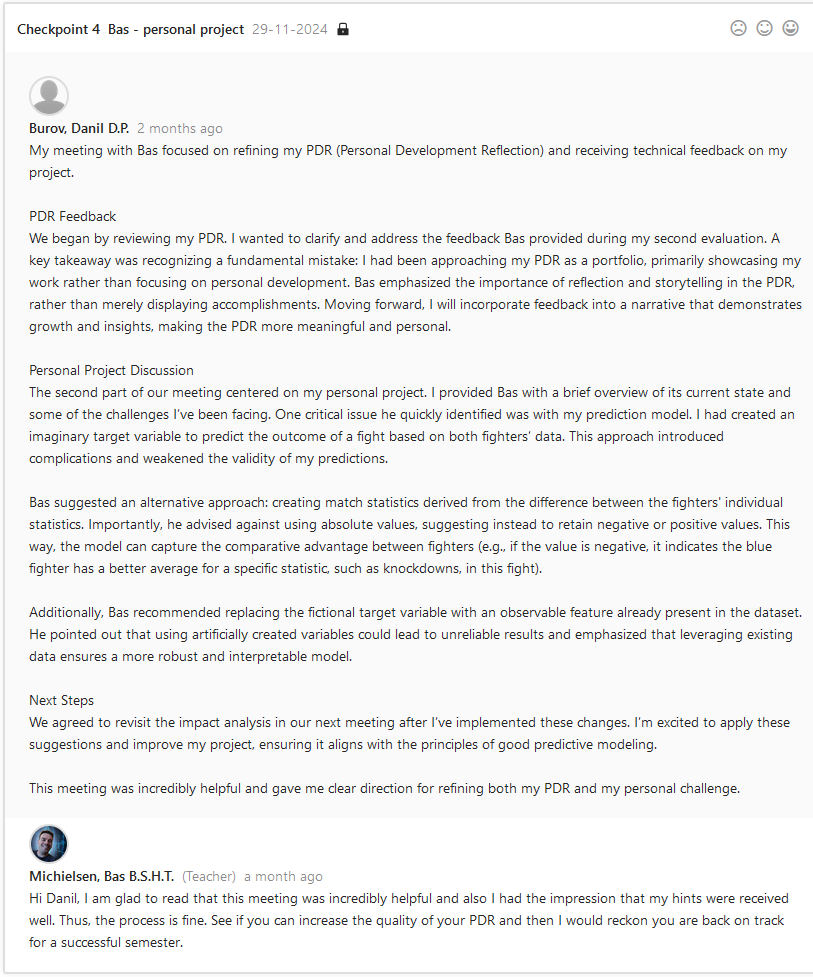
\includegraphics[width=\textwidth]{images/Feedback_Bas_1.png}
	\newpage
	Particularly from this feedback I am talking about the 'Personal Project Discussion' where I mention that I had created an imaginary target variable.\\\\
	\underline{Self assesment: Proficient}
\section{Learning outcome 5 - Data visualization}
\underline{\textbf{Description}}\\
The student is able to use data to create an interesting, informative and 
compelling story in an (interactive) data visualization product, tailored to the right target group.\\
\underline{\textbf{Explanation:}}\\
Visualizing data will help further understand the relation between different features. In order to achieve this goal,
every correlation found between different features needs to be visualized. These images need to be understandable and 
self-explanatory.

\subsection{First evaluation}
I have not yet done anything related to data visualization. I have only educated myself with the provided Python tutorials and self-learning.\\
\underline{\textbf{Self assessment: Orientating}}

\subsection{Second evaluation}
I have been able to visualize the correlations with the features for my project. Unfortunately, the correlations are not that strong and I fear that 
the data is very unaccurate and that is making the data show this information. In the future I would like to find correlations for my personal project, answering 
the question which fighter statistics make the percentage of a fighters' chance of winning higher. \\\\
\underline{\textbf{Self assessment: Beginning}}

\subsection{Third evaluation}
Unfortunately, I have not received specific feedback on my data visualizations. However, I did create several plots for both my personal project and my group project. Through this process, I began to appreciate the value of visualizations in gaining deeper insights into data. While Bas and I briefly reviewed my visualizations, we didn’t delve deeply into them. Based on the feedback I received for data preparation, I recognize that my visualizations can be significantly improved.\\

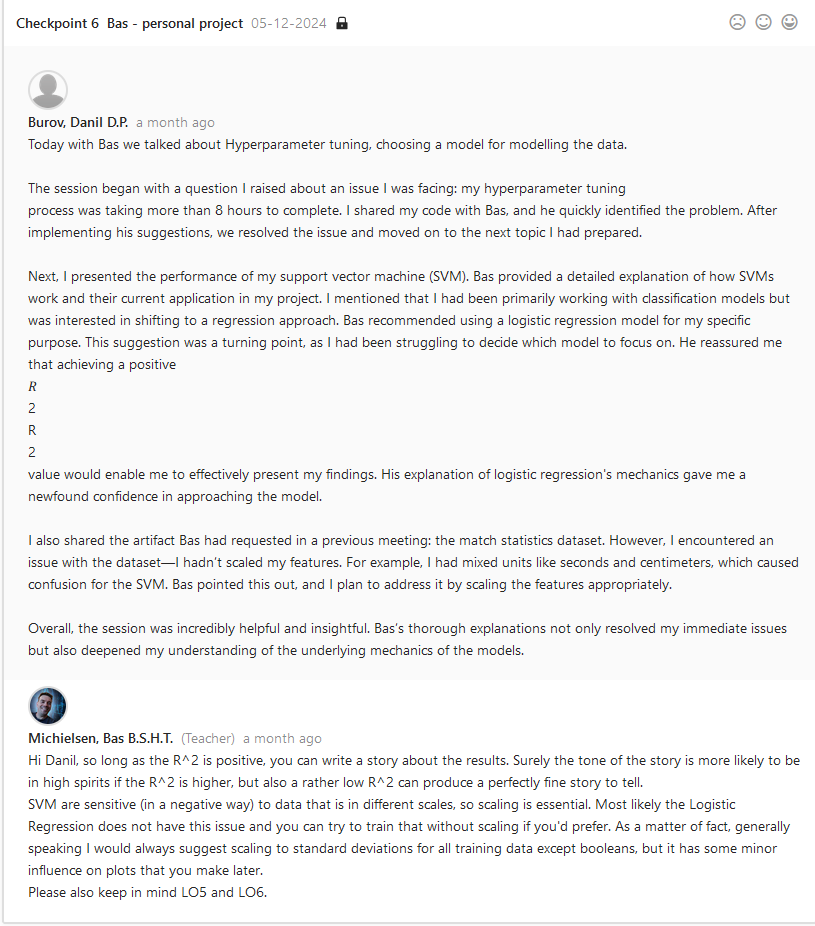
\includegraphics[width=\textwidth,keepaspectratio]{images/Feedback_Bas_2.png}\\

One of the key issues is that I did not apply standard deviation to my dataset, which led to inaccuracies in my plots. This oversight highlights the importance of ensuring data is properly prepared before creating visualizations, as any errors in the dataset will inevitably affect the clarity and accuracy of the resulting visuals.\\

Looking ahead, I want to engage in discussions with Bas and other technical consultants to better understand which types of plots would best suit my personal project. I also aim to learn how to interpret these visualizations effectively to maximize their value. By refining this skill, I hope to leverage data visualization as a powerful tool for both analysis and communication\\
  \underline{\textbf{Self assessment: Beginning}}
\subsection{Final evaluation}
This learning outcomes was one of my main focuses for improvement during the final quarter of the minor. During this quarter I made a lot of different visualization that give me a better understanding of my data and helped me model it to a better level. I found that making visualization is not as easy as I thought, because an image need to have a clear message to the reader, however it needs to support the point you are trying to convey. An image can convey a thousand words, however, it could lead to misunderstanding if it is unclear.
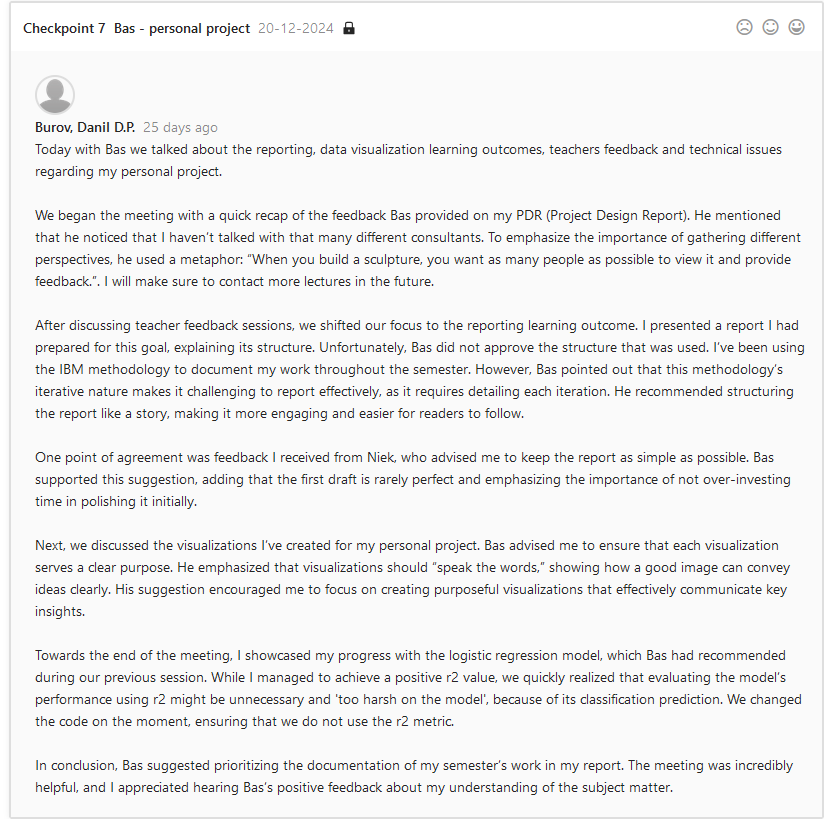
\includegraphics[width=\textwidth,keepaspectratio]{images/Feedback_Bas_3.png}\\
Because of this feedback, I was reminded what an image should show and how I should integrate it in my reports.\\\\
Although, I did create quite a few visualization I did not explain them further in my python notebook which led to confusion for some of my plots. This was done given the feedback I received when Bas had a look of my visualization.
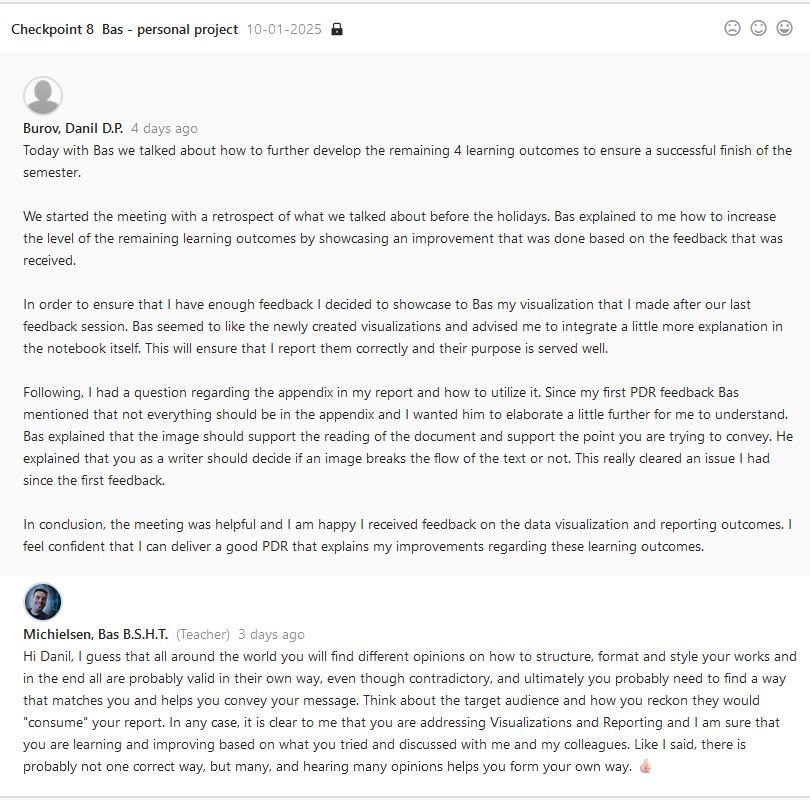
\includegraphics[width=\textwidth,keepaspectratio]{images/Feedback_Bas_4.png}\\\\
\underline{Self assesment: Proficient}

\section{Learning outcome 6 - Reporting}
\underline{\textbf{Description}}\\
The student is able to report in a methodologically sound manner on (the outcome of) 
their own AI projects (project proposal, process documentation, reporting of final results, etc.).\\
\underline{\textbf{Explanation:}}\\
It is important that documents are written in time and feedback is used to prove the legitimacy of the given goal. The goal would be considered 
accomplished if all documents are consistent and comprehensible. It is very important that the code documentation is easy
to understand and use.

\subsection{First evaluation}
It is essential for me to document the progress I make in order to keep track of how I have improved during the minor. To do so, 
I have created my own personal repository where I have already put all the documents I have written up until now, as well as all the exercises 
I have completed over the past few weeks.\\\\
\underline{\textbf{Self assessment: Beginning}}

\subsection{Second evaluation}
I have added markdown 'README' file in my repository to make everything more structured and to be easily found. I am trying to work as transparently as
possible and document the work I do. In order to keep it transparent I write markdown in the python notebooks,ensuring that everything I do is 
understandable and comprehensive.\\\\
Link to my personal repository: \href{https://github.com/BurovDanil/MinorAI}{Personal repository for the minor}\\
Link to my personal project notebook: \href{https://github.com/BurovDanil/MinorAI/blob/main/PythonCR/Personal%20project/UfcModel.ipynb}{Personal project notebook}\\
Link to my group project notebook: \href{https://github.com/AI-Farming-Thewi/cows_analysis/blob/stagri-farm-analysis/Stagri%20analysis.ipynb}{Group project notebook}\\\\
\underline{\textbf{Self assessment: Proficient}}

\subsection{Third evaluation}
Since the beginning of the semester, I have been focusing on documenting my work to improve my reporting skills. To support this effort, I have experimented with different tools to record the progress and results of my work. Seeking a professional perspective on how to align these efforts with my personal goals, I consulted with Niek. He advised me that as long as a document has a clear purpose, it can effectively showcase my learning process.\\
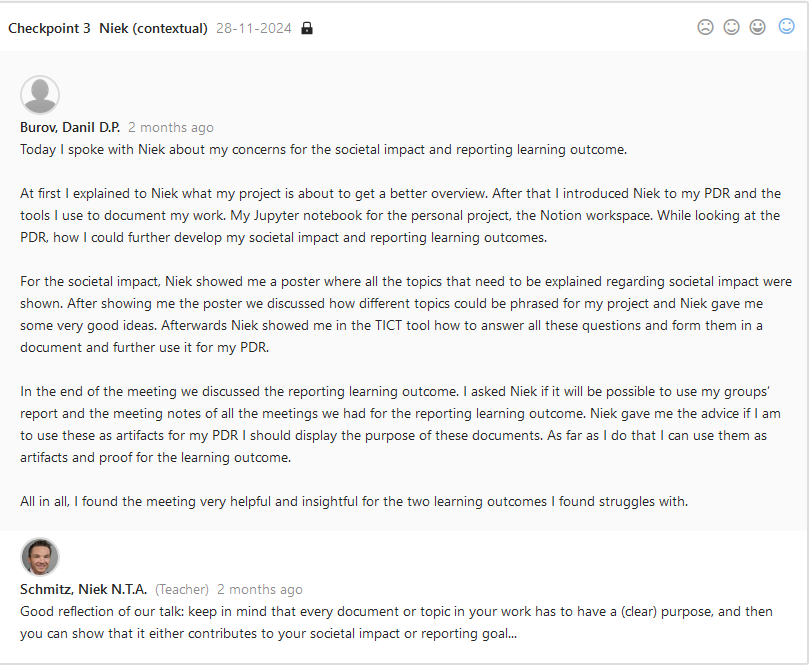
\includegraphics[width=\textwidth,keepaspectratio]{images/Feedback_Niek_1.png}\\

This advice made me reconsider my approach. Instead of using all the documentation material I had created separately, I decided to compile a well-rounded document that integrates all my work throughout the minor. When I shared this idea with Niek, he supported it and provided additional guidance. He emphasized that a good report doesn’t have to be lengthy; a concise, well-structured document can often be more impactful. This insight surprised me but left a lasting impression.\\
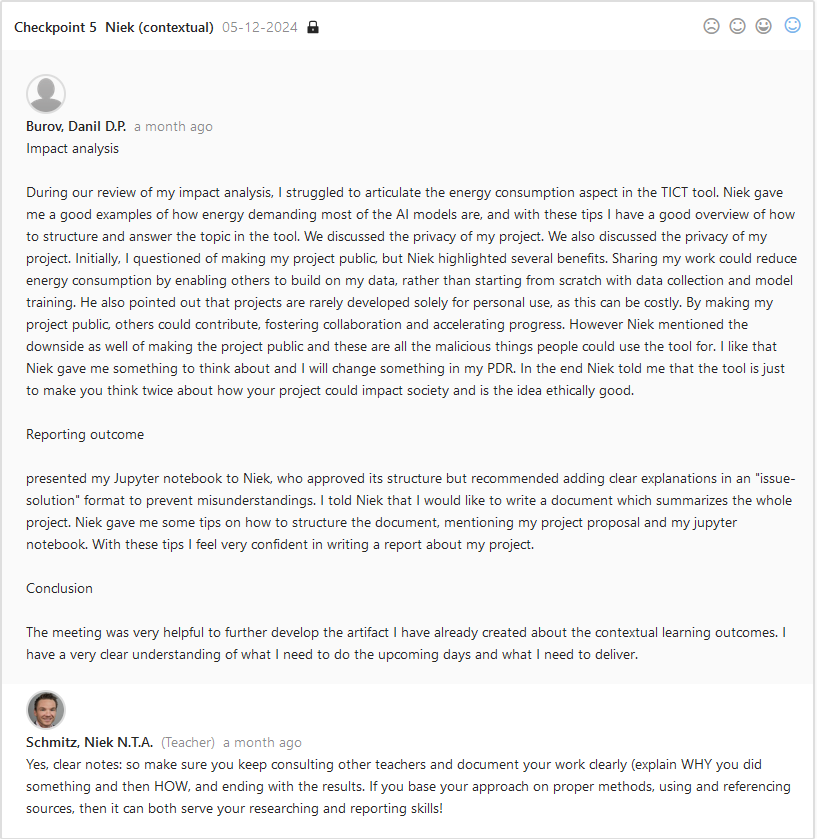
\includegraphics[width=\textwidth,keepaspectratio]{images/Feedback_Niek_2.png}\\

My plan now is to consolidate all my project documentation into a clear and structured report. Even if the final outcome of the project isn’t entirely positive, I want to create a document that effectively communicates the work I have done and is easy for others to read and understand.\\
  \underline{\textbf{Self assessment: Beginning}}
\subsection{Final evaluation}
\underline{Self assesment: Proficient}

\section{Learning outcome 7 - Personal Leadership}
\underline{\textbf{Description}}\\
The student shows an entrepreneurial mindset regarding their own AI project(s) and personal development, while being aware
of their own learning capacity and keeping in mind professional ambitions in their future work field.\\
\underline{\textbf{Explanation:}}\\
The outcome of this learning goal should be that I manage my time correctly without overloading myself. That means following some kind of a schedule, 
as well as attending lectures to ensure that I stay on track and seeking feedback to make sure I am progressing.

\subsection{First evaluation}
Ever since the minor started, I have attended all lectures regarding the minor and have taken some insights that will help me further develop my skills in AI modeling. 
I still need to improve on asking for more feedback from lecturers.
\underline{\textbf{Self assessment: Orientating}}

\subsection{Second evaluation}
I have been following a sort of strict schedule when it comes down to work. I am working from the morning to the late afternoon every Tuesday and Thursday
with my group. That way I ensure that I am always up-to-date with what my teammates are doing in the project. Moreover, I do my personal project work on Monday and Wednesday, leaving 
Friday to be a day which is free. This was done intentionally, making sure that if I feel that something needs more work I can do it then. \\\\
\underline{\textbf{Self assessment: Proficient}}
\subsection{Third evaluation}
Since the last evaluation, I have adjusted my approach to personal leadership. I now prioritize incorporating feedback into my workflow, organizing my week around regular feedback sessions. For example, I schedule a feedback session every Thursday, ensuring that I deliver the results from the previous session by that day.

This approach has proven to be highly efficient. It keeps me focused, encourages consistent progress, and helps me accomplish more within a structured timeframe. Additionally, working closely with my tutors allows me to keep them updated on my progress, fostering better collaboration and alignment with my goals.\\
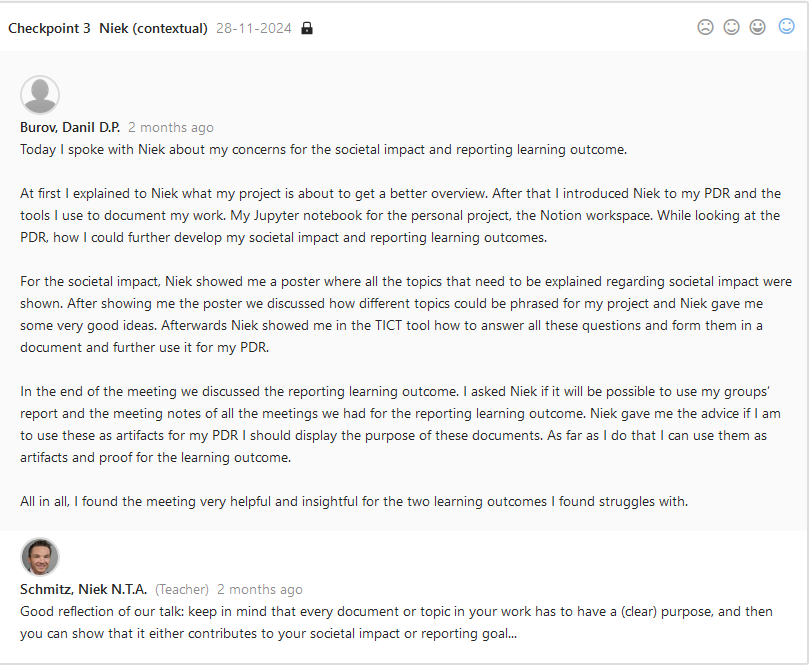
\includegraphics[width=\textwidth,keepaspectratio]{images/Feedback_Niek_1.png}\\
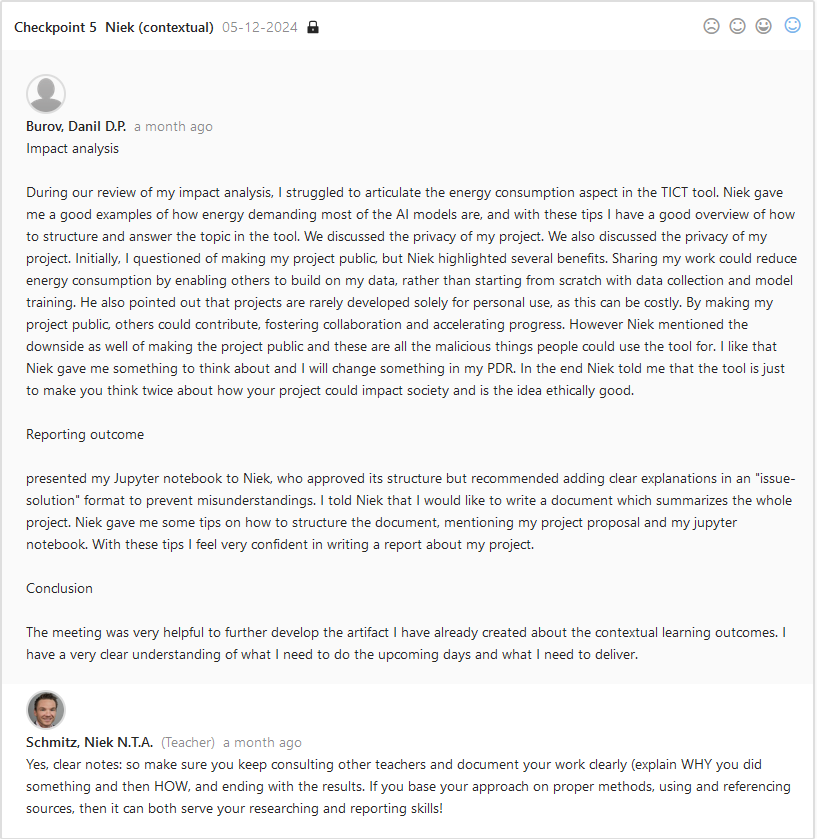
\includegraphics[width=\textwidth,keepaspectratio]{images/Feedback_Niek_2.png}\\
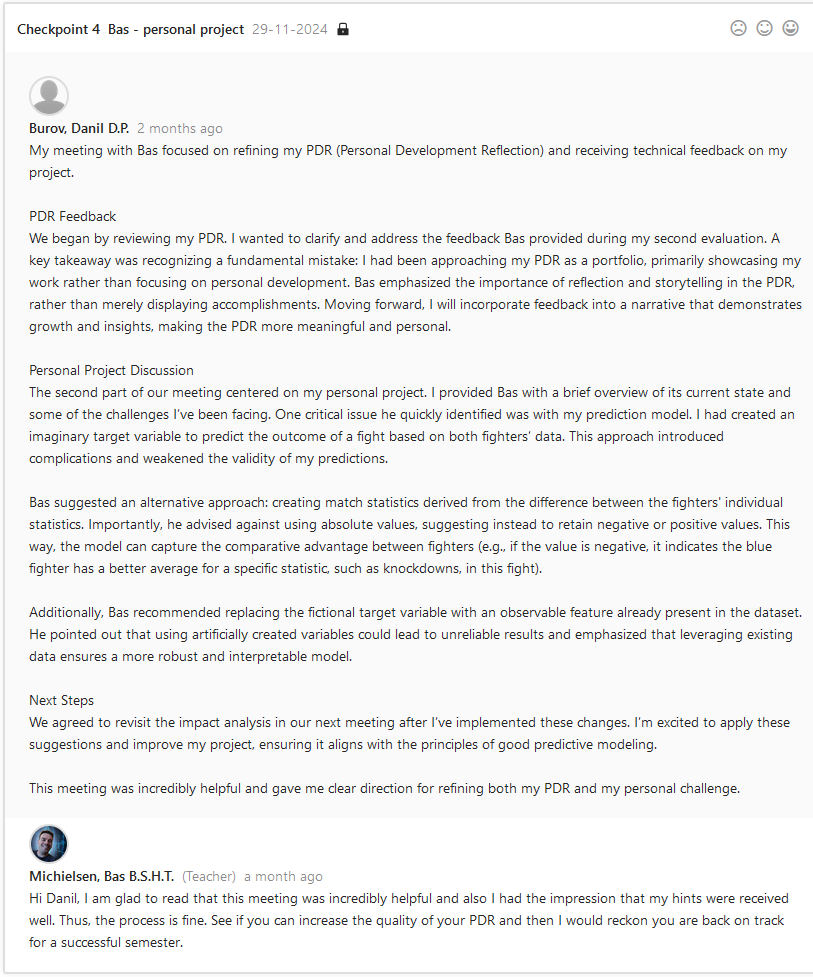
\includegraphics[width=\textwidth,keepaspectratio]{images/Feedback_Bas_1.png}\\
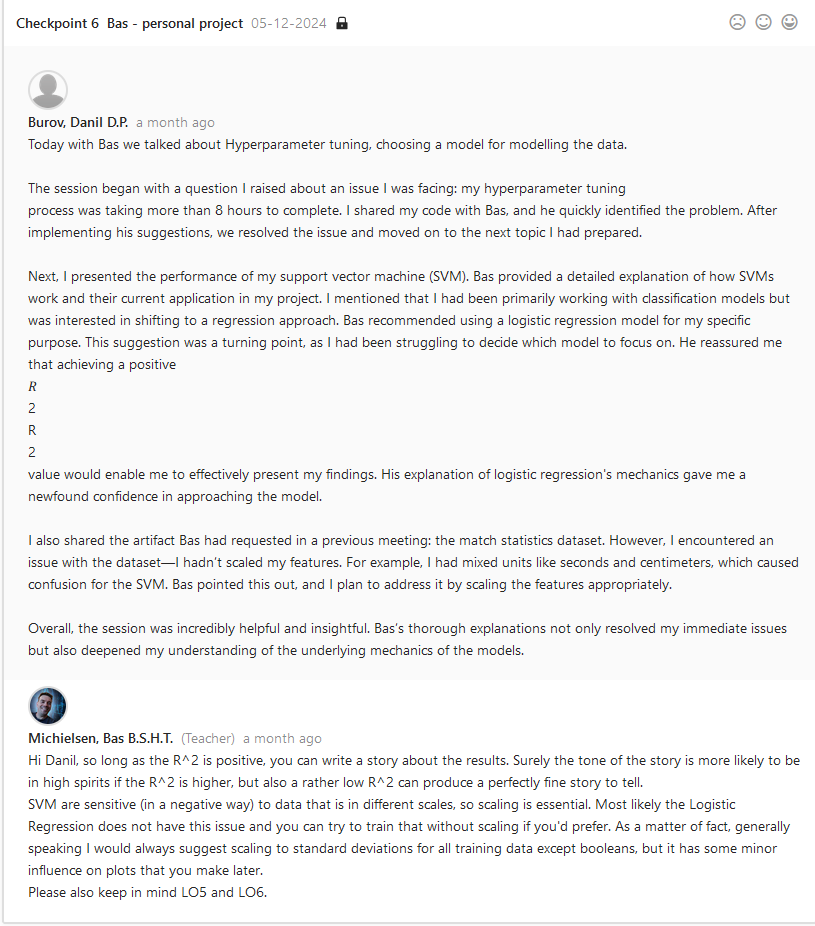
\includegraphics[width=\textwidth,keepaspectratio]{images/Feedback_Bas_2.png}\\
  \underline{\textbf{Self assessment: Beginning}}
\subsection{Final evaluation}
I have continued with the same workflow to ensure a strong finish for the last quarter of the semester. However, due to the holidays I did not manage to get that many feedback sessions, however I think I have received enough feedback to finish the semester with a positive outcome.\\
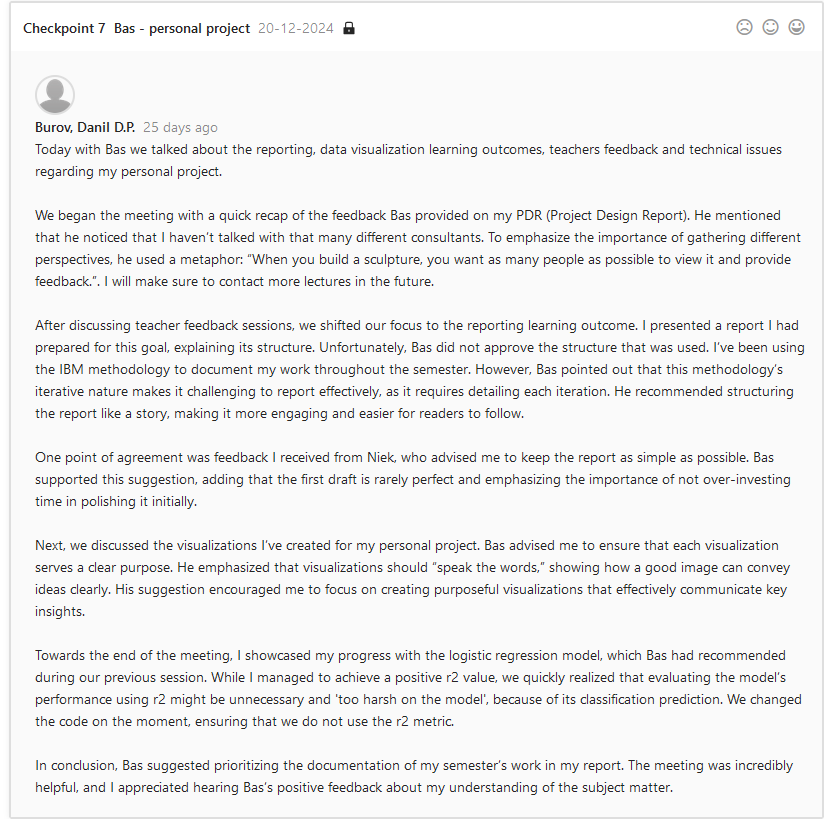
\includegraphics[width=\textwidth,keepaspectratio]{images/Feedback_Bas_3.png}\\
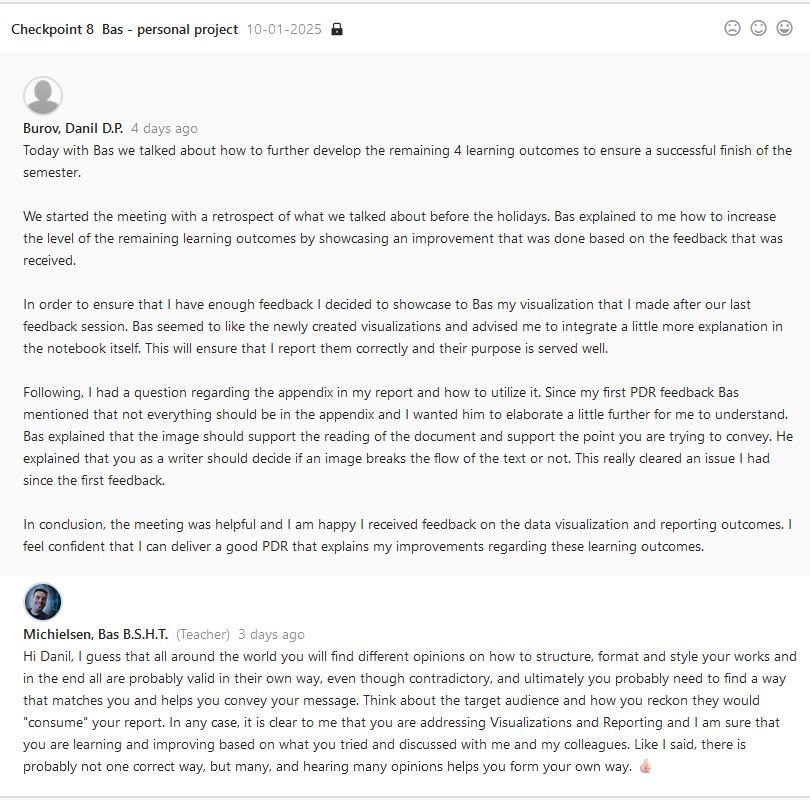
\includegraphics[width=\textwidth,keepaspectratio]{images/Feedback_Bas_4.png}\\\\
%ADD NIEK FEEDBACK HERE
\underline{Self assesment: Proficient}

\section{Learning outcome 8 - Personal goal}
\underline{\textbf{Description}}\\
With this learning outcome, the student can set their own goal in relation to their future field of work.
This is always related to your Individual Challenge. Describe this Learning Outcome in your PDR.

\underline{\textbf{Explanation:}}\\
My personal goal for this minor is to become very familiar with how to create an AI model, be able to analyze large amounts of data,
and prepare this data for further training of a given model. I would like to get more familiar with how machine learning algorithms work 
and be able to choose the appropriate algorithm for the use case.

\subsection{First evaluation}
In the first 4 weeks, I managed to choose a dataset for my personal project that fits my needs. I attended all lectures to make 
sure I progress in my knowledge of AI, both technically and ethically. I managed to import the dataset and clean it based on a condition.

\underline{\textbf{Self assessment: Orientating}}

\subsection{Second evaluation}
From week six to nine I believe that I have progressed quite a lot since the previous four weeks. I have done a lot of data preparation for 
modelling and even managed to train my first model. I am very content with the work I have done regarding my personal project, tackling legal issues 
as well battling accuracy in the moment. I know that the current dataset may not be enough to train a model sufficiently as well, so I am very excited for the 
upcoming weeks and how both my projects will progress. I am currently getting familiar with different machine learning algorithms since I found not much 
success in my personal projects' model I am currently using.
\subsection{Third evaluation}
Regarding my personal goal, I feel confident in saying that I have made significant progress in approaching the creation of AI models, managing large datasets, and selecting the appropriate model for the data's purpose.\\
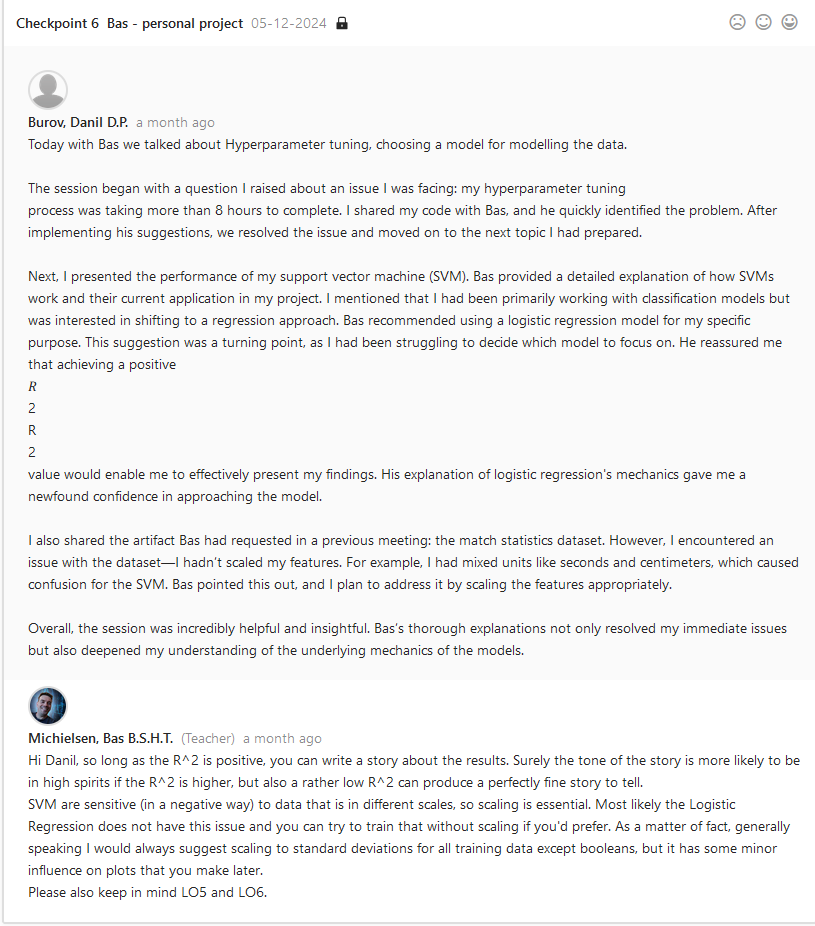
\includegraphics[width=\textwidth,keepaspectratio]{images/Feedback_Bas_2.png}\\
Reflecting on the feedback I have received, I realize how much my knowledge has expanded throughout this process. Engaging in discussions about various models with Bas, presenting my cleaned dataset, and receiving constructive feedback have all contributed to my growth. These moments not only highlight my learning but also reinforce the progress I have made toward achieving my goals.\\
  \underline{\textbf{Self assessment: Beginning}}
\subsection{Final evaluation}
I think that my progress for the semester is significant. I have familiarized myself with concepts I did not know before. I am happy that I managed to get to a level where I can talk freely about data preparation, machine learning algorithms, etc. with my coach and my teammates. It can be clearly seen in this feedback how the different data science terminology is used when discussing a problem with my semester coach Bas. I am very proud of myself and thankful to my coach that he gave me always a different point to explore after each feedback session. This really improved my learning curve by a lot!\\
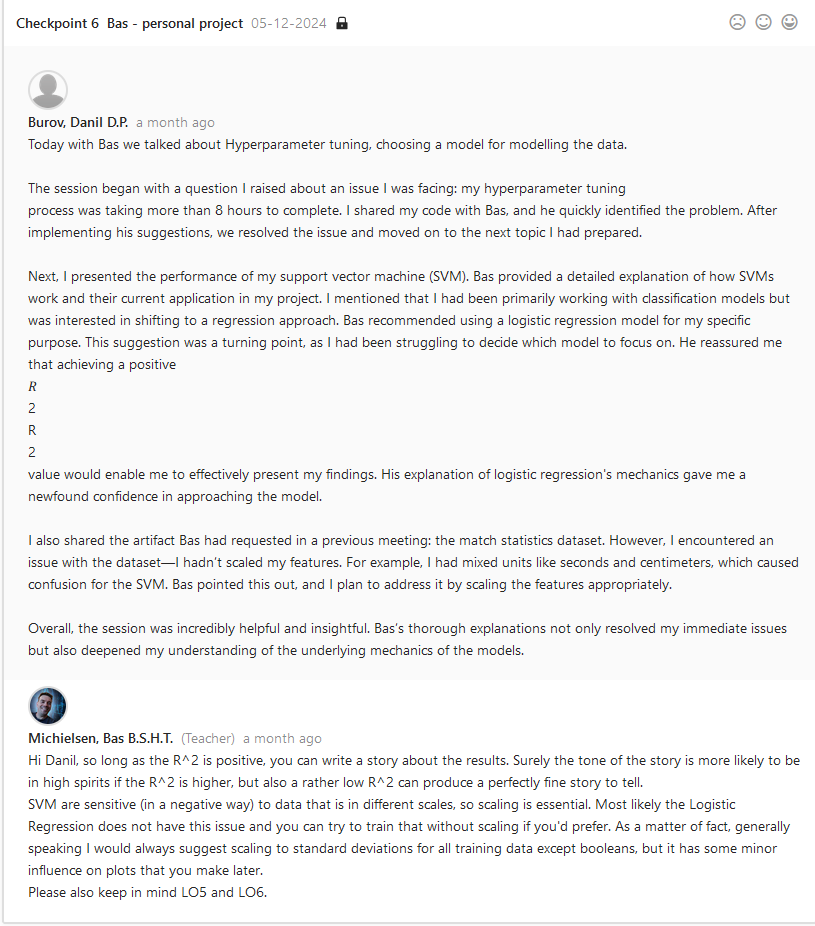
\includegraphics[width=\textwidth,keepaspectratio]{images/Feedback_Bas_2.png}\\\\
\underline{Self assesment: Proficient}

\section{Retrospect} % ONLY IN FINAL VERSION
Looking back at all the evaluations the only thing I can say is that it was quite the experience! From not knowing what AI is to calculating $r^2$ and analysing and combining datasets. From having no idea what could possibly be a societal impact to creating a whole document explaining the different impacts my project could have on society, further developing my analytical skills. From being unsure if I can achieve my personal goal to wanting to add more to it because of the possibilities I found while learning about AI. I am very proud of myself that I managed to establish such a good foundation of data science skills and if I want I could continue developing my career into this field!
\section{Conclusion} % ONLY IN FINAL VERSION
I came in this minor without any prior knowledge about data science or any terminology for AI whatsoever, and now being able to understand news about the AI world and getting myself even more familiar with the hottest topic of the world feels truly empowering! Even though, the semester is at an end I will continue evolving my skills in the data science field of IT. This minor gave me such a good foundation to continue exploring this world and I feel enthusiastic doing so!
\end{document}
